To achieve the desired outcome, we need to modify the original code by removing the spiral-like layers of arcs and replacing them with three concentric circles, each containing two labeled arcs. Here's an example of how you can do this using TikZ:
```
\documentclass{article}
\usepackage{tikz}
\begin{document}
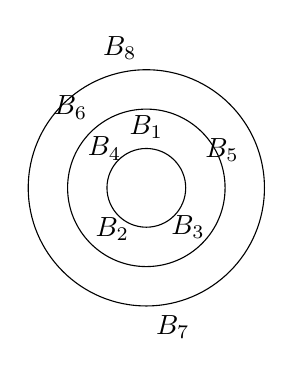
\begin{tikzpicture}
  % Define the radius of the innermost circle
  \def\radius{0.5cm}
  
  % Draw the innermost circle
  \draw (0,0) circle (\radius);
  
  % Label the first arc on the innermost circle
  \node at (90:\radius) [anchor=south] {$B_1$};
  
  % Label the second arc on the innermost circle
  \node at (210:\radius) [anchor=north] {$B_2$};
  
  % Define the radius of the middle circle
  \def\radius{1cm}
  
  % Draw the middle circle
  \draw (0,0) circle (\radius);
  
  % Label the third arc on the middle circle
  \node at (330:\radius) [anchor=east] {$B_3$};
  
  % Label the fourth arc on the middle circle
  \node at (150:\radius) [anchor=west] {$B_4$};
  
  % Define the radius of the outermost circle
  \def\radius{1.5cm}
  
  % Draw the outermost circle
  \draw (0,0) circle (\radius);
  
  % Label the fifth arc on the outermost circle
  \node at (30:\radius) [anchor=north east] {$B_5$};
  
  % Label the sixth arc on the outermost circle
  \node at (150:\radius) [anchor=south west] {$B_6$};
  
  % Label the seventh arc on the outermost circle
  \node at (270:\radius) [anchor=north west] {$B_7$};
  
  % Label the eighth arc on the outermost circle
  \node at (90:\radius) [anchor=south east] {$B_8$};
\end{tikzpicture}
\end{document}
```
This code will produce a circle with three layers of arcs,